\begin{frame}{Effects of Sublimation within a Crater}

\begin{figure}
\centering

\begin{subfigure}{0.48\textwidth}
    \centering
    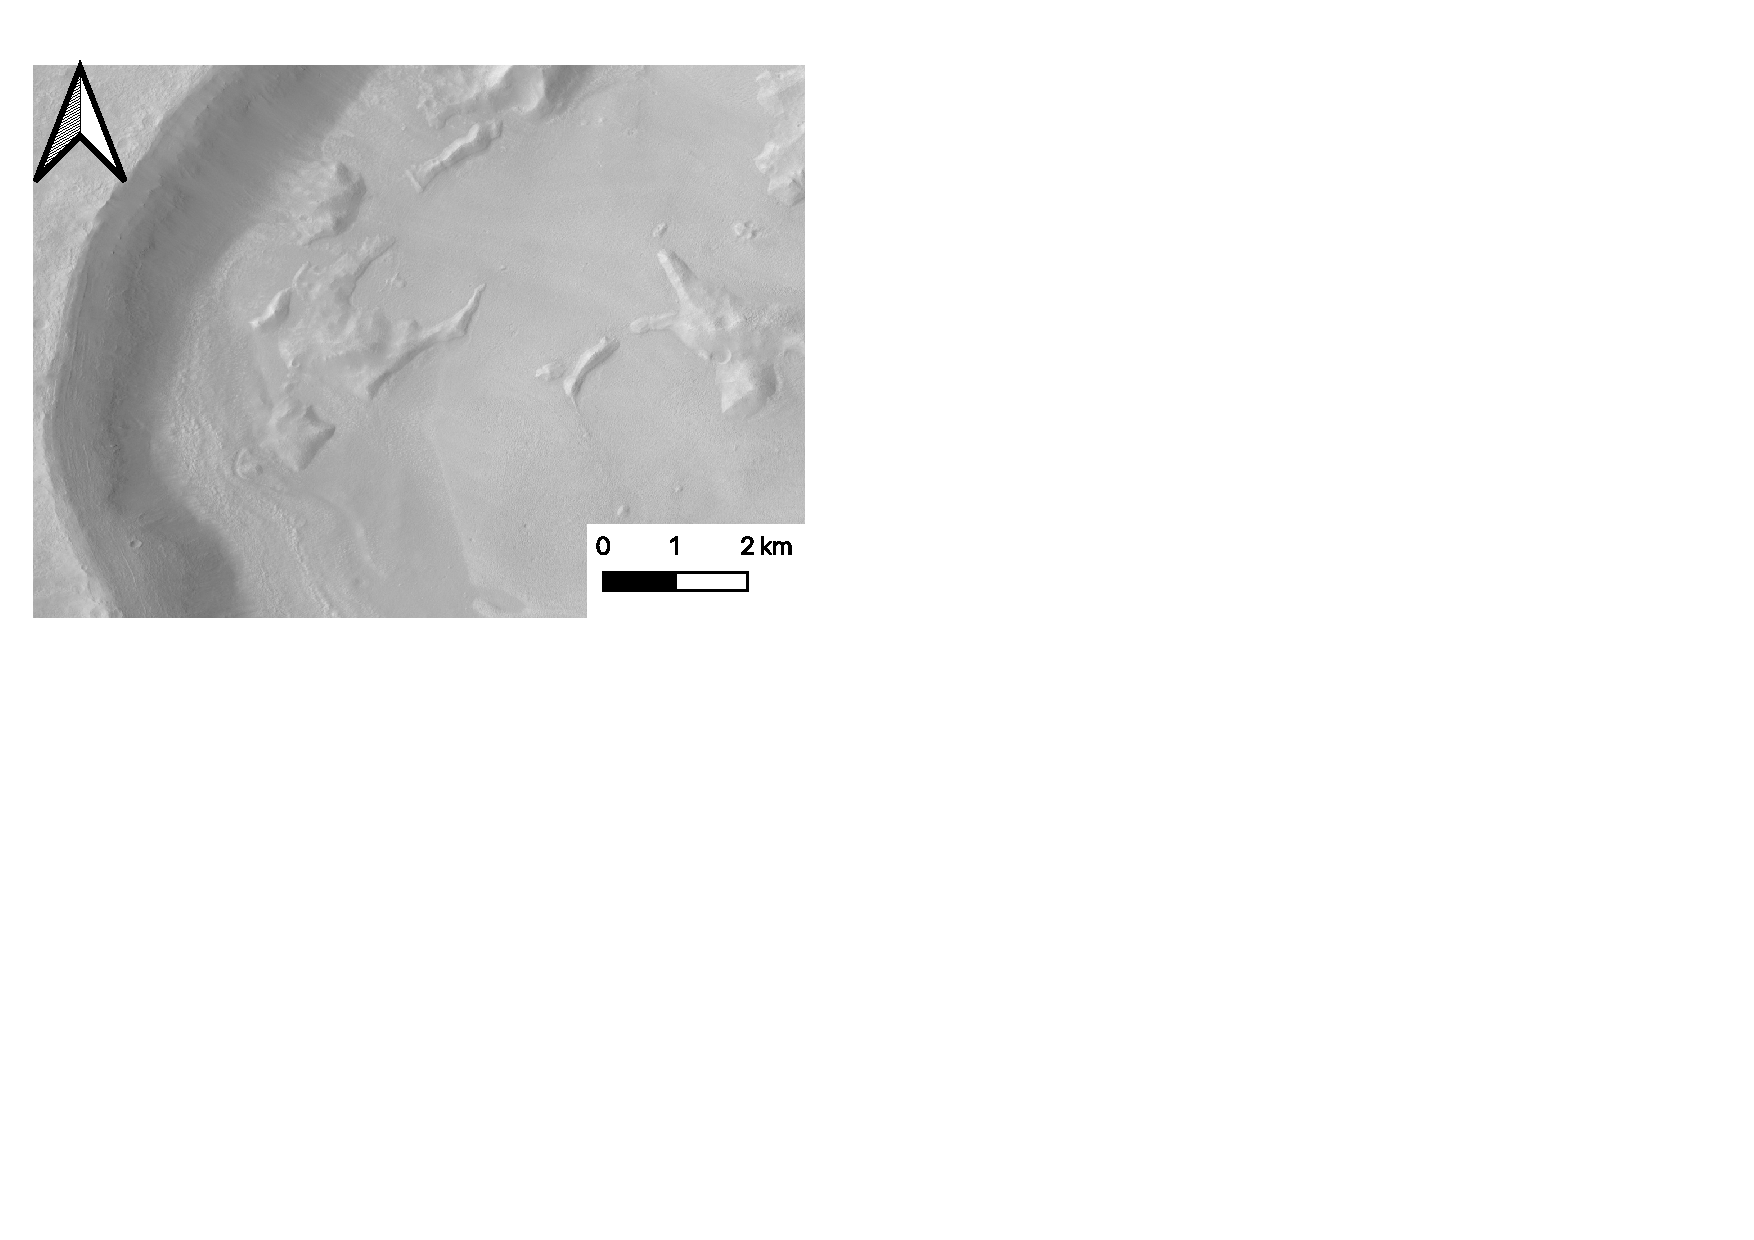
\includegraphics[
        width=\linewidth,
        height=0.65\textheight,
        keepaspectratio
    ]{Figures/CTX/CraterIce_Img.pdf}
    \label{fig:CraterIce_a}
\end{subfigure}
\hfill
\begin{subfigure}{0.48\textwidth}
    \centering
    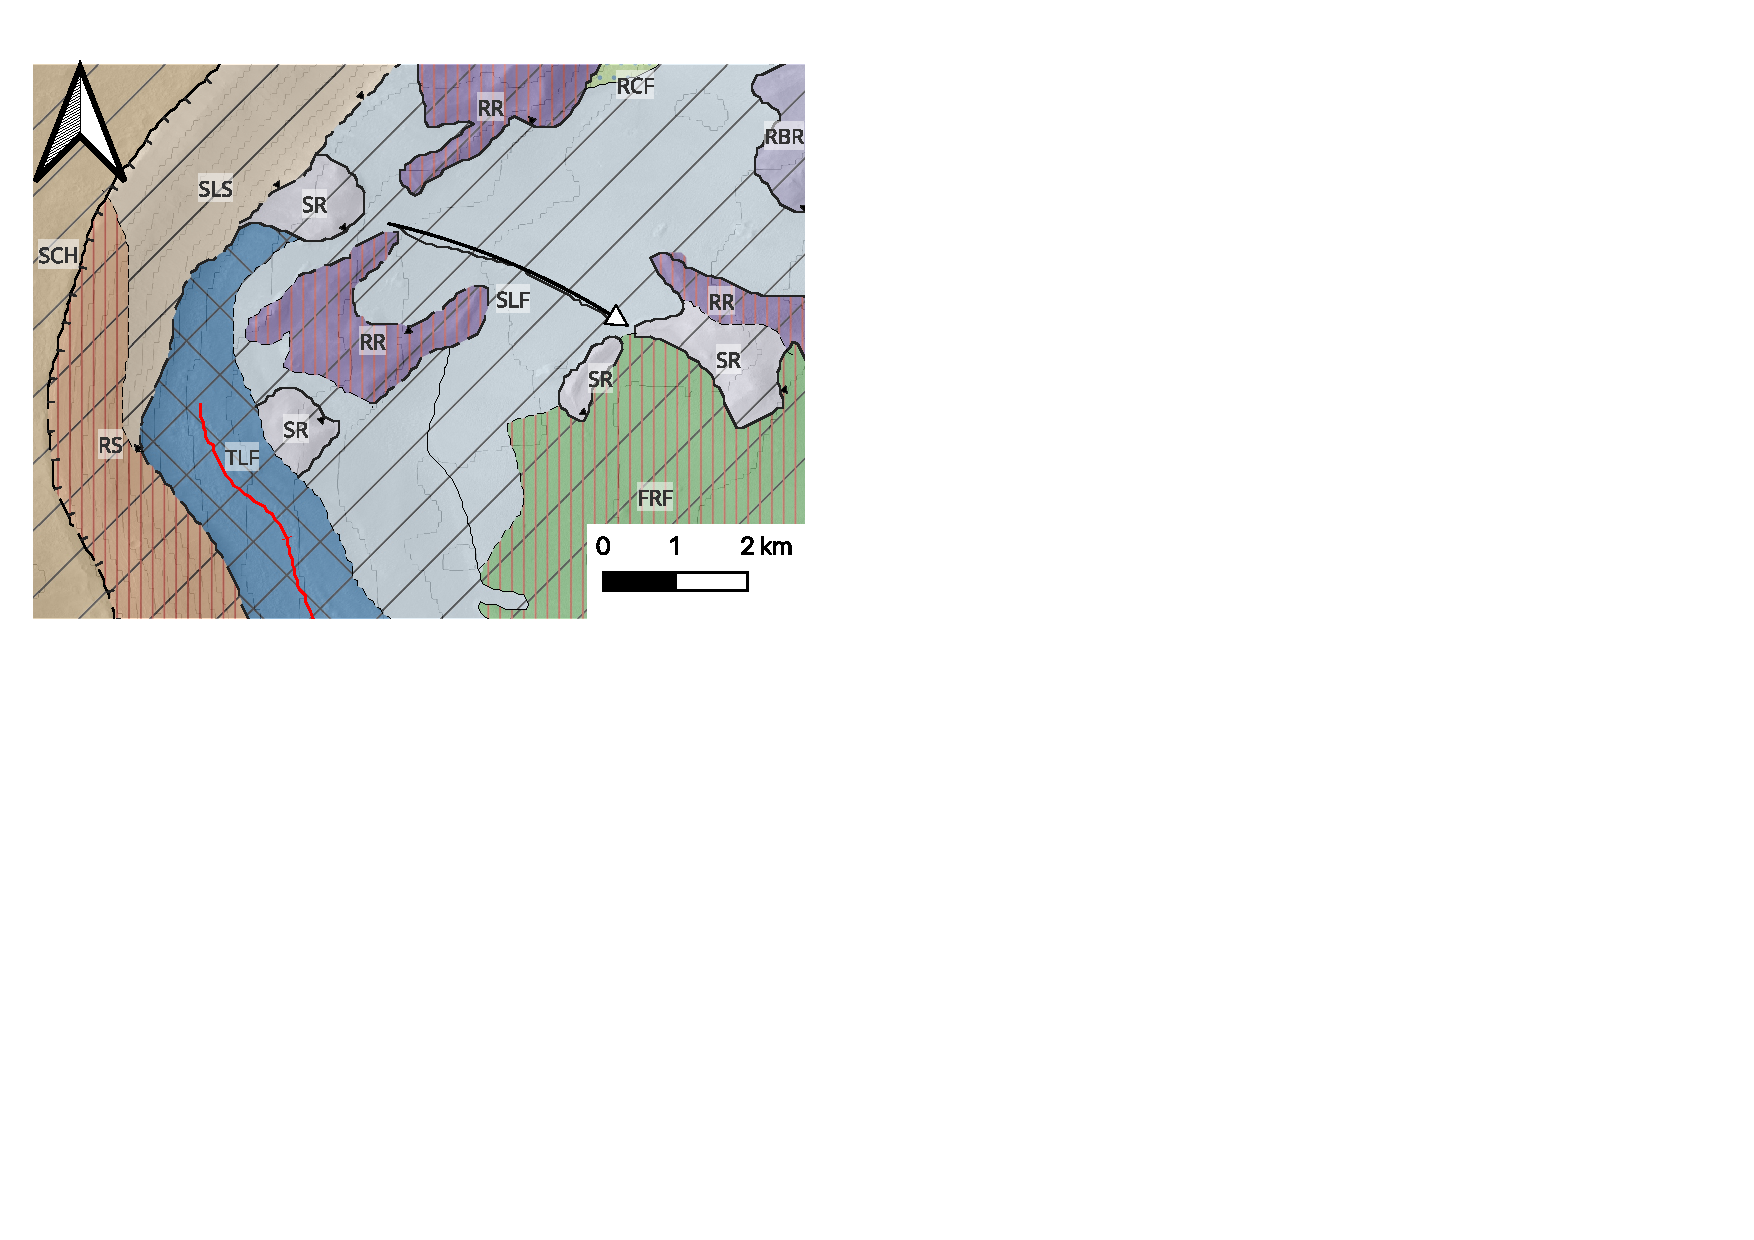
\includegraphics[
        width=\linewidth,
        height=0.65\textheight,
        keepaspectratio
    ]{Figures/CTX/CraterIce_Map.pdf}
    \label{fig:CraterIce_b}
\end{subfigure}

\caption{Crater containing concentric crater fill (CCF) and mesas (centred at $34.14375^{\circ}$N, $16.52417^{\circ}$E).}
\label{fig:CraterIce}

\end{figure}

\end{frame}

\againframe{LargeVFFs}
